%%%%%%%%%%%%%%%%%%%%%%%%%%%%%%%%%%%%%%%%%%%%%%%%%%%%%%%%%%%%%%%%%%%%
%%%%%%%%%%%%%%%%%%%%%%%%%%%%%%%%%%%%%%%%%%%%%%%%%%%%%%%%%%%%%%%%%%%%
%%                                                                %%
%% Esimerkki opinn�ytteen tekemisest� LaTeX:lla 20130926          %%
%% Alkuper�inen versio Luis Costa,  muutokset Perttu Puska        %%
%%                                                                %%
%% T�h�n esimerkkiin kuuluu tiedostot                             %%
%%               opinnaytepohja.tex (versio 1.7)                  %%
%%               aaltothesis.sty (versio 1.7)                     %%
%%               kuva1.eps                                        %%
%%               kuva2.eps                                        %%
%%                                                                %%
%%                                                                %%
%% K��nt�minen                                                    %%
%% latex:                                                         %%
%%             $ latex opinnaytepohja                             %%
%%             $ latex opinnaytepohja                             %%
%%                                                                %%
%%   Tuloksena on tiedosto opinnayte.dvi, joka                    %%
%%   muutetaan ps-muotoon seuraavasti                             %%
%%                                                                %%
%%             $ dvips opinnaytepohja -o                          %%
%%                                                                %%
%% Selitt�v�t kommentit on t�ss� esimerkiss� varustettu           %%
%% %%-merkeill� ja muutokset, joita k�ytt�j� voi tehd�,           %%
%% on varustettu %-merkeill�                                      %%
%%                                                                %%
%%%%%%%%%%%%%%%%%%%%%%%%%%%%%%%%%%%%%%%%%%%%%%%%%%%%%%%%%%%%%%%%%%%%
%%%%%%%%%%%%%%%%%%%%%%%%%%%%%%%%%%%%%%%%%%%%%%%%%%%%%%%%%%%%%%%%%%%%

%% modified Aalto Master Degree Thesis tamplate
%% author Liu Peng


%% Use one of these you write in Finnish:
%% the 1st when using pdflatex (use pdf figures) or
%% the 2nd when producing a ps file (use eps figures).
%\documentclass[finnish,12pt,a4paper,pdftex]{article}
%\documentclass[finnish,12pt,a4paper,dvips]{article}


%% Uncomment one of these if you write in English
\documentclass[english,12pt,a4paper,pdftex]{article}
%\documentclass[english,12pt,a4paper,dvips]{article}

%% This package is required
%% Choose your school from arts, biz, chem, elec, eng, sci.
%% Choose the character encoding scheme used by your editor: utf8, latin1
%\usepackage[elec,utf8]{aaltothesis} % this is the default in aaltothesis.sty
\usepackage[elec,latin1]{aaltothesis}


%%
%% Use this if you run pdflatex and use jpg/pdf-format pictures.
%%
\usepackage{graphicx}
\usepackage{subfigure}
\usepackage{titlesec} 

%% Use the macros in this package to change how the hyperref package below 
%% typesets its hypertext -- hyperlink colour, font, etc. See the package
%% documentation. It also defines the \url macro, so use the package when 
%% not using the hyperref package.
%\usepackage{url}


%% Use this if you want to get links and nice output with pdflatex
\usepackage[pdfpagemode=None,colorlinks=true,urlcolor=red,%
linkcolor=blue,citecolor=black,pdfstartview=FitH]{hyperref}


%% Use this if you write hard core mathematics, these are usually needed
\usepackage{amsfonts,amssymb,amsbsy}  

%% Vaakasuunnan mitat, �L� KOSKE!
\setlength{\hoffset}{-1in}
\setlength{\oddsidemargin}{35mm}
\setlength{\evensidemargin}{25mm}
\setlength{\textwidth}{15cm}
%% Pystysuunnan mitat, �L� KOSKE!
\setlength{\voffset}{-1in}
\setlength{\headsep}{7mm}
\setlength{\headheight}{1em}
\setlength{\topmargin}{25mm-\headheight-\headsep}
\setlength{\textheight}{23cm}


%% add chapter title depth to 4, use paragraph to represent subsubsubsection
\setcounter{secnumdepth}{4}
\titleformat{\paragraph}
{\normalfont\normalsize\bfseries}{\theparagraph}{1em}{}
\titlespacing*{\paragraph}
{0pt}{3.25ex plus 1ex minus .2ex}{1.5ex plus .2ex}


%% Output starts heref
\begin{document}


%% Change the school field to describe your school if the autimatically 
%% set name is wrong
% \university{aalto University}{aalto-Yliopisto}
% \school{School of Electrical Engineering}{S�hk�Tekniikan korkeakoulu}


%% Only for B.Sc. thesis: Choose your degree programme. 
%\degreeprogram{Electronics and electrical engineering}%
%{Elektroniikka ja s�hk�tekniikka}
%%


%% Only for M.Sc. and Licentiate thesis: Choose your department,
%% professorship and professorship code. 
\department{Department of Communications and Networking}%
{Radiotieteen ja -tekniikan laitos}
\professorship{Networking Technology}{Piiriteoria}
\code{S-38}
%%


%% Choose one of these:
%\univdegree{BSc}
\univdegree{MSc}
%\univdegree{Lic}


%% Should be self explanatory...
\author{Peng Liu}

%% Your thesis title. If the title is very long and the latex 
%% does unsatisfactory job of breaking the lines, you will have to
%% break the lines yourself with \\ control character. 
%% Do not hyphenate titles.
\thesistitle{Developing a Solution for Multimedia Home Networking}{ }

\place{Espoo}

%% For B.Sc. thesis use the date when you present your thesis. 
\date{20.5.2015}


%% B.Sc. or M.Sc. thesis supervisor 
%% Note the "\" after the comma. This forces the following space to be 
%% a normal interword space, not the space that starts a new sentence. 
\supervisor{Prof.\ Raimo A. Kantola}{Prof.\ Raimo A. Kantola}


%% B.Sc. or M.Sc. thesis advisors(s). 
%%
%% Note that there has been a change in the official EN translation
%% of the Finnish title ``ohjaaja'' which in the previous version (1.5) 
%% of this document was called ``instructor''. The recommended
%% translation is now ``advisor''.  
%% However, the LaTeX internal variable remains \instructor
%% as there is little point to change the variable name. 
%%
%\instructor{Prof. Pirjo Professori}{Prof. Pirjo Professori}
\instructor{D.Sc.\ (Tech.) Mikko Valimaki}{TkT Olli Ohjaaja}
%\instructor{M.Sc.\ (Tech.) Polli Pohjaaja}{DI Polli Pohjaaja}


%% Aalto logo: syntax:
% \uselogo{aaltoRed|aaltoBlue|aaltoYellow|aaltoGray|aaltoGrayScale}{?|!|''}
%% Logo language is set to be the same as the document language.
\uselogo{aaltoRed}{''}


%% Create the coverpage
\makecoverpage


%% Force new page so that English abstract starts from a new page
\newpage
%
%% English abstract, uncomment if you need one. 
%% 
%% Abstract keywords
\keywords{Home network, Multimedia, HTTP Streaming,\\ UPnP, DLNA, Miracast, AirPlay}
%% Abstract text
\begin{abstractpage}[english]

%% Abstract chapter
%% author Liu Peng

 This thesis analyzes the solutions to home multimedia networking, compares 
 nowadays-popular home networking solutions, especially for the Digital Living
 Network Alliance standard. By comparing different features and
 implementations, our team developed a suitable mobile solution for multimedia
 home networking which takes advantage of both Airplay,  DIAL and DLNA
 protocols on Android platform.

 It started with a comparison of popular streaming technologies, Airplay, 
 DLNA, Miracast and Chromecast. By analyzing the features and capabilities 
 of those streaming technologies, we proposed a universal solution for 
 multimedia home networking by supporting multiple protocols and building
 bridge to different platforms.

 In the middle of the thesis, I tested different multimedia solutions and 
 we implemented a mobile Application for home networking on Android. The
 architecture, features and analyze methodology are discussed in the paper. We
 also investigate how to bridge home networking and Internet resources, an
 online channel proxy is made in our app "Streambels" to stream online
 channels like YouTube. Finally we got a published Android application for
 Tuxera Inc. The application is already published in Google Play Store for 6
 months, which generate a statistic report of how users use our app, so there
 is a short description of the user behavior, and how we could improve user
 experience by analyzing these data.

 At the end of the paper there is a discussion on the possible further
 development and the future of Home network.

\end{abstractpage}
%% Note that 
%% if you are writting your master's thesis in English place the English
%% abstract first followed by the possible Finnish abstract

%% Preface
%\mysection{Esipuhe}
\mysection{Preface}

%% Preface chapter
%% author Liu Peng

This document is my master's thesis of \textit{Communications Engineering majoring in
Networking} at Aalto University. All research and development of this thesis was
conducted at Tuxera Inc. in Helsinki from January 2013 to June 2014. Tuxera is a
high-tech startup that develops kernel-level file systems and multimedia solutions
for leading software, hardware and electronics companies.\\
\\
During this project I worked together with my colleagues at Tuxera, I started
to work on DLNA project for the first few months during which period I learned
DLNA architecture and made a research about Digital Media Server solutions.
After that I worked on an Android project to develop a universal solution for
multimedia home networking.
\subsection*{Acknowledgements}
First of all, I would like to thank the Streambels team at Tuxera, whom I worked
together throughout the project. I would like to thank Karthik Ramakrishna, our
lead developer. Every week he helped solving problems in the project,
no matter the question was theoretical or technical, he always answered my
questions. As our project manager, Oscar Santolalla helped us with
organizational problems we encountered and taught us to look at things from a
end user perspective as well. Sakari Tanskanen, our mobile developer helped us
by integrating Chromecast and FireTV support to Stremabels. Nadir Javed, our
quality assurance engineer helped us with the quality management and testing of
potential bugs before releasing the product to end users. Karolina Mosiadz, our
Public Relations Manager helped to listen to user's feedback every day and provide the unique
insights in improving Streambels. Hien Le, our UX designer helped us to develop
a very handy user interface. And special thanks to Mikko Valimaki and Szabolcs
Szakacsits who lead the company and gave me the opportunity to participate in
this great project. Without them, I would not have been able to finish this
report.\\
\\
I thank my university supervisor Raimo Kantola, who helped me to develop a good
thesis topic based on my project and helped me with initial problem description.
I got great support from him with his critique and useful advice, especially
during the middle and final period, when I wrote the report.\\
\\
Finally, I thank everybody who supported me during my graduation work,
especially my family, friends and house-mates.

\vspace{1.5cm}
%\vspace{5cm}
Otaniemi, 20.5.2015

\vspace{5mm}
{\hfill Peng\ Liu \hspace{1cm}}


%% Force new page after preface
\newpage


%% Table of contents. 
\thesistableofcontents


%% Symbolit ja lyhenteet
%%
%% Symbols and abbreviations
%\mysection{Symbolit ja lyhenteet}
\mysection{Abbreviations}

%% Abbreviations chapter
%% author Liu Peng

%\subsection*{Symbolit}
\subsection*{Symbols}

\begin{tabular}{ll}

\end{tabular}

%\subsection*{Operaattorit}
\subsection*{Opetators} 

\begin{tabular}{ll}

\end{tabular}

%\subsection*{Lyhenteet}
\subsection*{Abbreviations}

\begin{tabular}{ll}
DLNA       & Digital Living Network Alliance \\
DMC        & Digital Media Controller \\
DMS        & Digital Media Server \\
DMR        & Digital Media Renderer \\
HTTP       & HyperText Transfer Protocol \\
RTSP       & Real Time Streaming Protocol \\ 
DRM        & Digital Rights Management \\ 
\end{tabular}


%% Corrects the page numbering, there is no need to change these
\cleardoublepage
\storeinipagenumber
\pagenumbering{arabic}
\setcounter{page}{1}


%% Leip�teksti alkaa
%%
%% Text body begins. Note that since the text body
%% is mostly in Finnish the majority of comments are
%% also in Finnish after this point. There is no point in explaining
%% Finnish-language specific thesis conventions in English.
%\section{Johdanto}
\section{Introduction}

%% Ensimm�inen sivu tyhj�ksi
%% 
%% Leave first page empty
\thispagestyle{empty}

%% Introduction chapter
%% autor Liu Peng

\subsection{Home networking}
People's lives are being digitalized. Home multimedia devices nowadays such as digital TVs,
smart phones, digital cameras, tablets, PCs, laptops and NAS (Network Attached
Storage) are all being equipped with ever greater processing power and mass storage, wielding the power  to
 record our daily lives and handle these multimedia informations. The digitalized world has also seen a rapid growing of network deployment. According to a research
\cite{stateofHN} done in 2011, in this industrialized world, networking
is being rapidly adopted at homes; for example, in the U.S. in 2009,
approximately 63\% of homes had gained access to a broadband connection. Over 50\% had even installed their own "home network", which is defined as multiple computers or devices sharing a broadband
 connection via either a wired or wireless connection within the home. In a typical
home scenario, most of these devices are connected to a local network such as a
Wi-Fi hot spot, in order to allow musics, pictures, videos and other content to
be ported across different devices.

\subsection{Problem description}
While the adoption of home networks has steadily increased since the late 1990s
and early 2000s, the home networks has indeed encountered problems and limitations
\cite{stateofHN}. For example, the usability of home-networking technologies has become
a key impediment to the adoption of new applications in the home, since the home-networking technology was originally developed for
 research labs and enterprise networks and does not account for the unique
 characteristics of home usage, such as the lack of professional administrators, deep
heterogeneity, and expectations of privacy.

Among all the challenges of home-networking, connecting all media devices and make them work together is getting increasingly interesting because of the rapid growth of consuming electronic market. Although there are
 several widely used multimedia-streaming solutions in the market, the 
standards employed are not compatible with each other. Furthermore, even devices using
the same standard are not always compatible with each other, due to the fact that the implementation approaches could vary from device to device. These incompatibilities have caused great inconvenience to the end users. 

DLNA, AirPlay, Chromecast and Miracast are the four major multimedia home network
digital living solutions. AirPlay is only used between Apple products; it
provides various features, including tunes play for music, AirPlay for video
and photos and screen mirroring. Miracast (previously called Wi-Fi display) was
proposed by Wi-Fi Alliance and has been receiving great popularity over the recent years.
Since its release version 4.2.2, Android has officially added the support for Miracast. In comparision, DLNA has been the most widely deployed solution so far, with 2.2 billion installations worldwide.
It was proposed by several industrial leading electronic manufacturers and network operators 
including AT$\&$T, Broadcom, Cisco, Google, Huawei, Intel, LG Electronics, Microsoft, Nokia, 
Panasonic, Samsung, Sony and Verizon.

As a result of different technical designs and  human aspects, these standards proposed by
different device manufactures naturally experience serious compatibility issues. It usually happens that
end users can have several multimedia-devices, with each one using a distinctive and unique  protocol, making it challenging or even impossible sometimes to share media between those devices. 

These compatibility issues has really obliged us to make a study on those multimedia-streaming
 technologies and to develop a more easy-to-use multimedia home networking solution
 with more  advanced technologies.

\subsection{Document overview}
The overview of popular home networking standards and solutions is described in
chapter 2(ref required). After a short comparison of these solutions, in chapter 3(ref required) we
describe a more universal solution for multimedia home networking and its
implementation. Chapter 4 presents some statistics from the Google Store
during the past few months. Besides, a study based on the user feedback
s is also presented. In Chapter 5, the paper is concluded by giving a discussion on the further development and prospect of home networking.
 

%% In a thesis, every section starts a new page, hence \clearpage
\clearpage

%\section{Aikaisempi tutkimus}
 \section{Background\label{chapter2}}
 
%% Background chapter 
%% author Liu Peng 
In recent years, the rapid development of electronics and computer science has
enabled home networking devices to become more affordable and more powerful. It
is currently common that a person may own several multimedia devices that
can be connected to the network.

Early research \cite{link_layer_old} \cite{end_user} \cite{link_layer}
conducted on home networking mainly aimed to find out how to build home
networking infrastructure. The subjects of the research, including cable
connection, wireless connection, and optical connection, concern more about
the physical layer of the home network.  So far, it has turned out that the
IEEE 802.11 protocol stack, among all others, is the most successful and 
widely deployed home networking infrastructure.

Currently, a typical scenario of home networking is that an IEEE 802.11
supportive wireless router connecting to an Ethernet cable, optical cable or
Asymmetric Digital Subscriber Line (ADSL) from the network operator creates
a local network and other user devices simply join this network. The wireless
Access Point (AP) employs the 802.11 b/g/n/ac protocol, utilizing the 2.4 GHz
or 5 GHz frequency channels and providing a 100+ Mbps  network connection,
whose bandwidth is sufficient for transmitting the popular High Definition
(1080p) videos.

In terms of network and application layer technologies, different device 
manufactures tend to choose their preferred multimedia-sharing protocols from
the pool of protocols that have been developed for a long time.

Since late 1990s, Universal Plug and Play (UPnP) protocol had been developed for
home networking usage \cite{upnp}. At that time, XML was popular and widely
used by different network applications. Under such background, UPnP was designed
to fully make use of XML. UPnP is independent of media types and devices, and it
runs on the TCP/IP stack, thus it can be easily applied to modern network
infrastructures.

In June 2003, Sony and several leading consumer electronic manufacturers
established the Digital Living Network Alliance (DLNA), a nonprofit 
collaborative trade association\footnote{\url{http://www.dlna.org/dlna-for-industry/our-organization}}. The
DLNA standard is based on the widely used UPnP protocol, but it added some
restrictions on media formats and some compatibility requirements. A device
hardware and software can be certified by DLNA organizations to prove that it
can work with other devices that also passed this certification.

In 2010, Apple quit DLNA and developed its own multimedia home networking 
solution, known as AirPlay\footnote{\url{https://www.apple.com/airplay/}}. By
adding screen mirroring, authentication and Remote Audio Output Protocol (RAOP)
music streaming, Apple tried to forge a more advanced home network sharing
system, aiming to provide a unique user experience among Apple products.
Apple's solution indeed attracted people's interest, and the user experience
proved much better than that of other similar products in the market. With its
improvement over the years,  Apple's solution has now been acknowledged as one
of the most popular streaming solutions.

Two years later, Wi-Fi alliance released its Miracast
technology\footnote{\url{http://www.wi-fi.org/discover-wi-fi/wi-fi-certified-miracast}},
and participated in pushing a new standard in wireless home networking. The
Miracast uses the Wi-Fi direct technology \cite{miracast_consumer} and it does
not require a wireless local network. Instead, a peer-to-peer connection is
created between the sharing and receiving devices. After its release, some
major software and hardware companies soon accepted this new standard. Google,
for example integrated Miracast support into its Android operating system, and
provided a screen-mirroring feature to other Miracast
receivers\footnote{\url{https://support.google.com/nexus/answer/2865484?hl=en}}.

The competition in home networking rages on over the years. In 2013, Google
released a 35-dollar
Dongle\footnote{\url{http://www.google.com/chrome/devices/chromecast/}}, using
its Chromecast protocol, which makes it possible to watch YouTube and Netflix
video directly on TV with such a dongle device. Laptop and mobile devices with
official YouTube App or Chrome browser can control the Dongle through the home
local network. In this solution, the home networking is pushed to the cloud,
since YouTube and Netflix content are directly downloaded from the Internet
whereas the mobile device just acts as a controller for choosing the
contents \cite{dial}.

At the same time, in September 2013, Spotify, a startup music service 
company also took part in making its own home networking solution, called 
Spotify Connect \cite{spotifyconnect}. Spotify Connect provides an interface for
users at home to access its huge music database, and directly browse and stream
using its mobile application. Home networking has again been pushed towards the
cloud and Internet services in Spotify Connect.

Since many companies would like to develop their own devices and even their 
own protocols, the market becomes disordered. Devices from different companies
are not compatible with each other, and users have to buy a different device in
order to access different services like Netflix and Spotify, which are provided
by different companies. This has created a significant demand on a solution that
can connect those devices at home and make them work together in a user friendly manner.

In response of this market need, the Streambels project has been initiated,
aiming to fill the gap among different protocols and connect these different
types of devices in the home networking environment.


\clearpage

\section{Developing a solution for multimedia home networking\label{chapter3}}

%% Developing a solution for multimedia home networking chapter
%% author Liu Peng

To fulfill the need of interoperability between devices in home networking,
Tuxera started a project called Streambels. Which aims to solve the
interoperability issue in multimedia home networking. The solution is to make a
combination of most popular solutions into one and connect all the resources
and displays in home. 

Since the hardware and networking settings are not easily changeable. And
nowadays smart phone has great CPU power and networking capability. It is well
adopted in people's home and even people's life. It is essential to develop a
mobile application that can be used to control all the multimedia data flow in
home networking. Through one year's development, our team developed an Android
application that can be used to control and connect every multimedia device in
the home. The application is integrated with a simple HTTP streaming server,
Airplay/ DLNA/ Chromecast/ FireTV device discovery, and
Airplay/ DLNA/ Chromecast/ FireTV streaming control point.

\subsection{Architecture overview}
The architecture of the solution is basically a combination of the most popular
solutions' solutions into one. The whole architecture contains three parts:
discovery, content management and streaming. 

Discovery component is responsible for device discovery which takes advantage of
both Multicast DNS and Simple Service Discovery Protocol. As discussed in
\ref{upnp}, the UPnP service uses Simple Service Discovery Protocol for device
discovery, the application firstly send a M-Search request over UDP to the
IPv4 multicast address 239.255.255.250 and UDP port 1900. Then the application
listen to other devices' response. DIAL devices will return a response with
Application URL header, while the UPnP/DLNA devices will return a message with
a XML body, which gives detailed service URL and description URL. SSDP is used
for both DLNA discovery and DIAL discovery. Multicast DNS is developed and
implemented by Apple Inc., and there is an open source implementation on its
website.

Content management component is responsible for organizing and
navigating multimedia contents which can be found in the home network. In our
solution, this includes both phone's local storage and DLNA digital media
servers that connected to home network. The sources can be used in all of the
three protocols that we support.

Streaming component is responsible for streaming multimedia content to selected
multimedia receivers, such as TVs, wireless speakers, set top boxes etc. In our
solution, since DLNA, AirPlay video/ photo and Chromecast all use HTTP streaming
while AirPlay music uses RTSP. Two types of media servers are built inside our
application. A RTSP server handles the AirPlay music streaming, a HTTP server handles all the
streaming else.

In order to serve media for all the receivers, two types of serve method need to
be implemented in a HTTP server. Since the DLNA guideline gave detailed
specification how the media file should be served on a HTTP server, the HTTP server should be
flexible to add DLNA specific headers, and should support byte based seeking
operation to enable "seek" action on the receiver side. For receivers other than
DLNA, a basic file server with byte range support will just do the work. After
comparing multiple server implementations on Android, NanoHTTPd is the perfect
library for our need, it is easy to use, Apache licensed, very tiny and
efficient implementation, since it is minimal implemented, so it is also easy to
be modified and add additional headers to be compatible with DLNA receivers.


A simplified version of our implementation is shown in the figure \ref{chart3}
below:
\begin{figure}[htb]
\centering 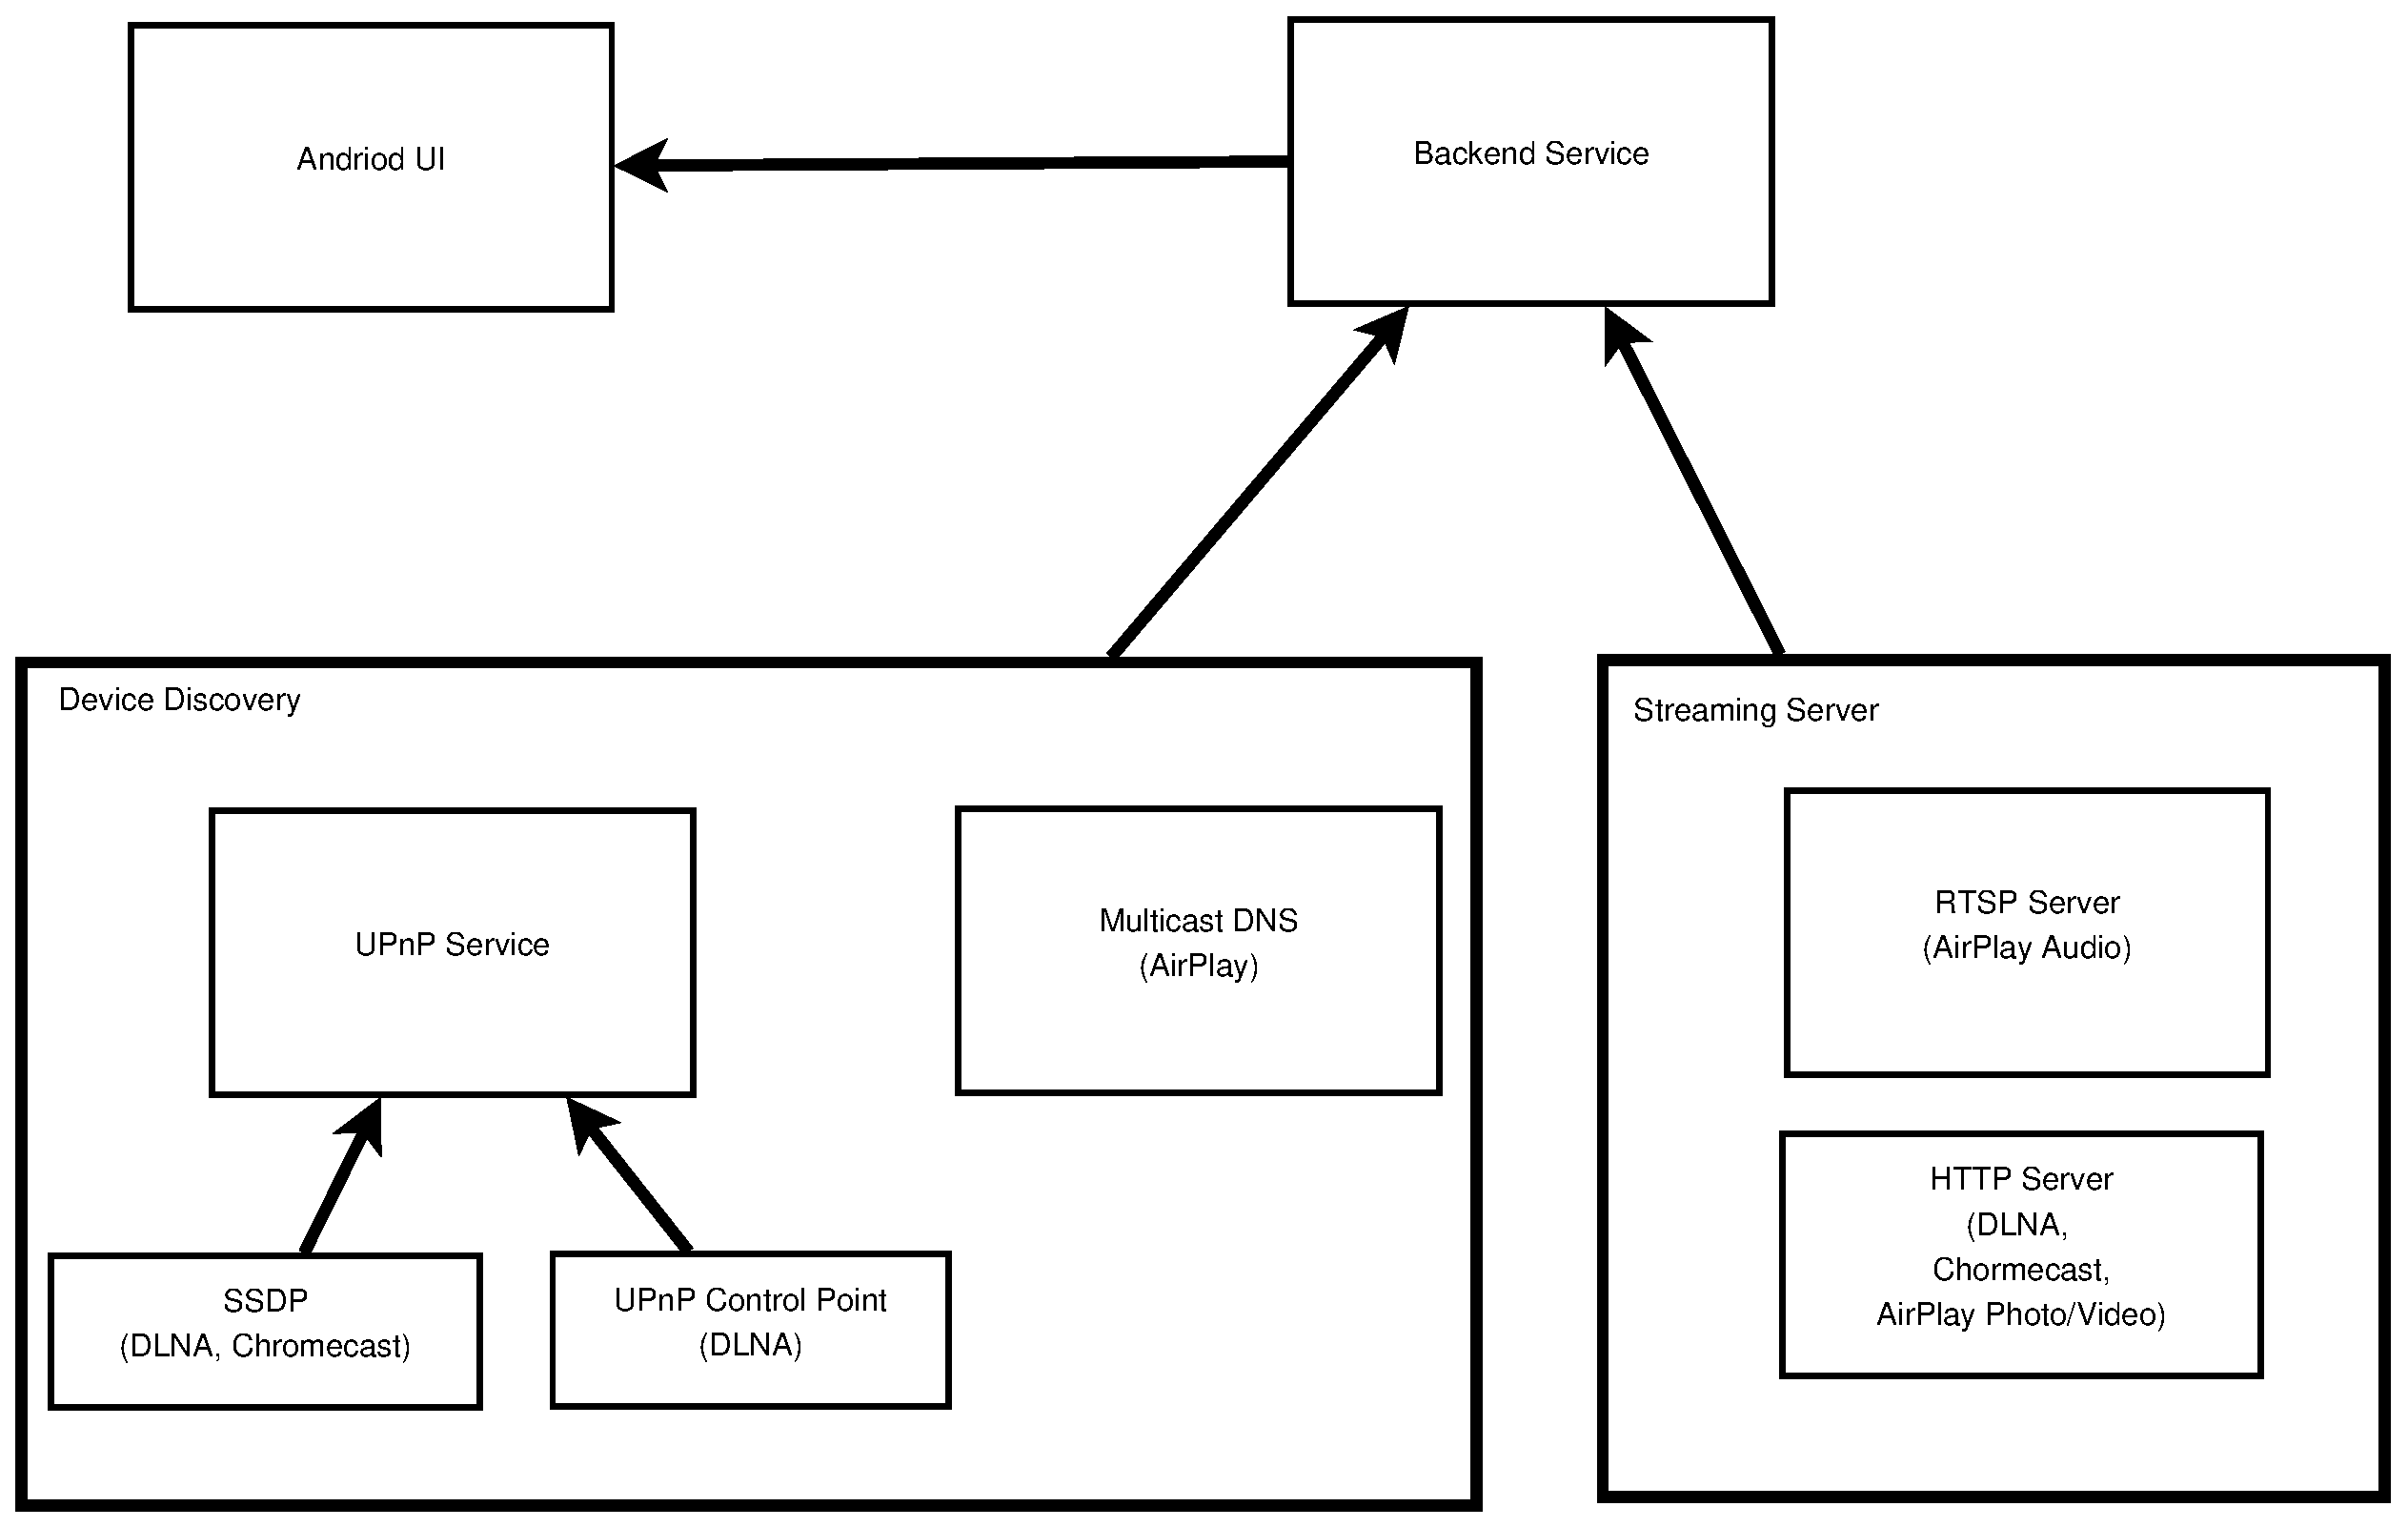
\includegraphics[height=9cm]{charts/chart3}
\caption{Simplified flow chart \label{chart3}}
\end{figure}

In terms of data flow, as described in figure \ref{chart4}, there are three
different types of data flow models: 

If the streamed content is stored in mobile phone, a streaming server in the
application is used to stream the content from phone to selected receiver.

Otherwise, if the content locates on the Internet, and the receiver is a DLNA
Media Renderer, a proxy is needed to firstly download the resource stream, add
the required headers by DLNA protocols and then stream the content to selected
DLNA Media Renderer.

Finally, if the streamed content locates in a DLNA Digital Media Server, the
source can be directly used by all receivers, in this case, the content
streaming happened directly from media server to receivers, application is only
used as a control point and do not participate in the media transmission.

\begin{figure}[htb]
\centering 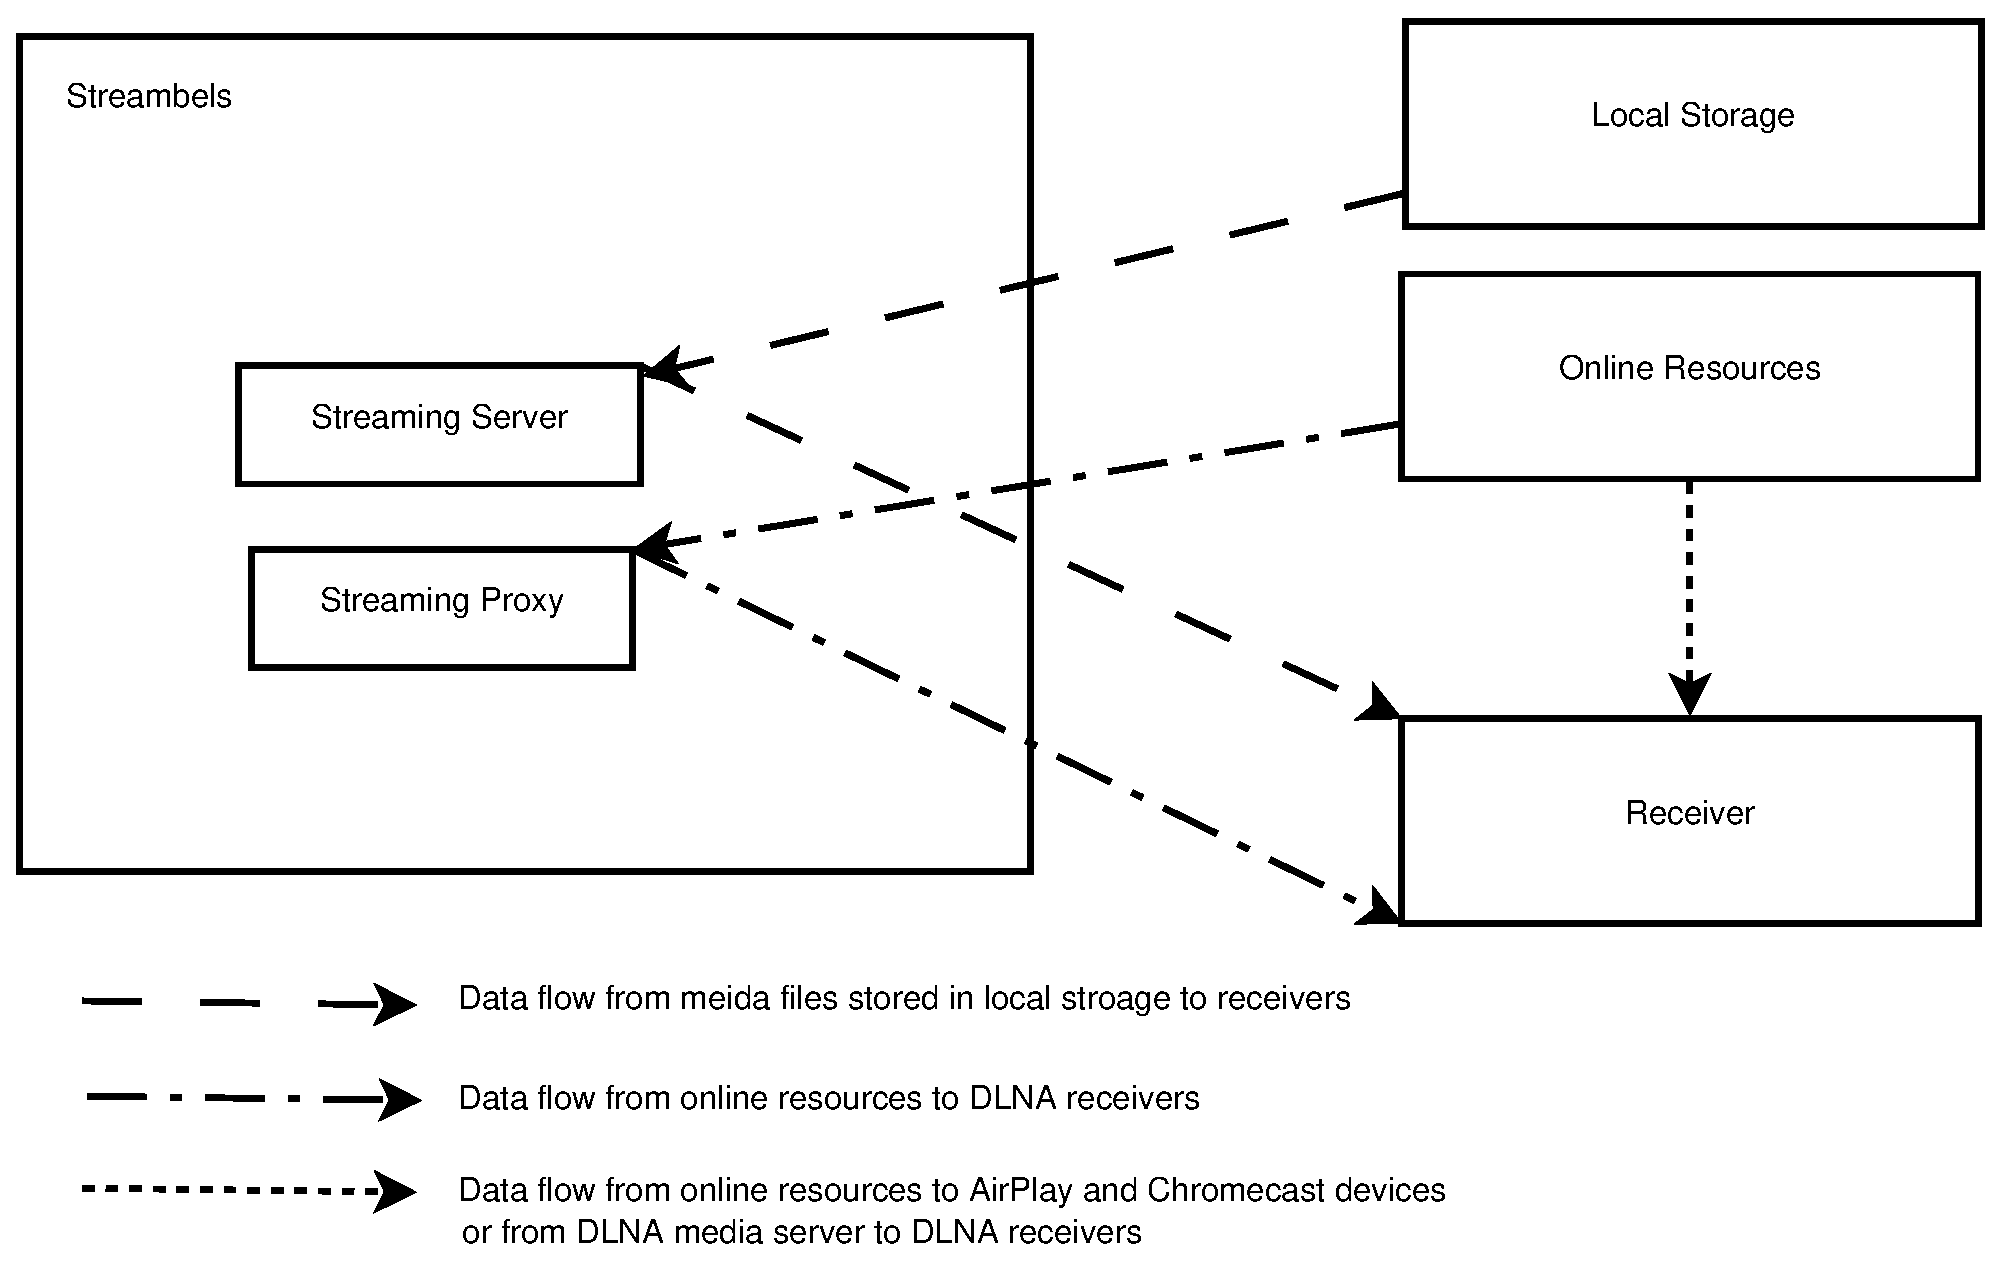
\includegraphics[height=9cm]{charts/data_flow}
\caption{Simplified data flow \label{chart4}}
\end{figure}

In terms of UI and UX, our designer Hien did a great job of defining a simple
and intuitive user interface \ref{chart5}, which benefits a lot for the user
experience.
In every place in the application, selected receiver is visible to user, it is also
visible as a button for switching between different receivers. 9 themes are also
available for users to select, which makes the application more fun to user.
\begin{figure}[htb]
\centering 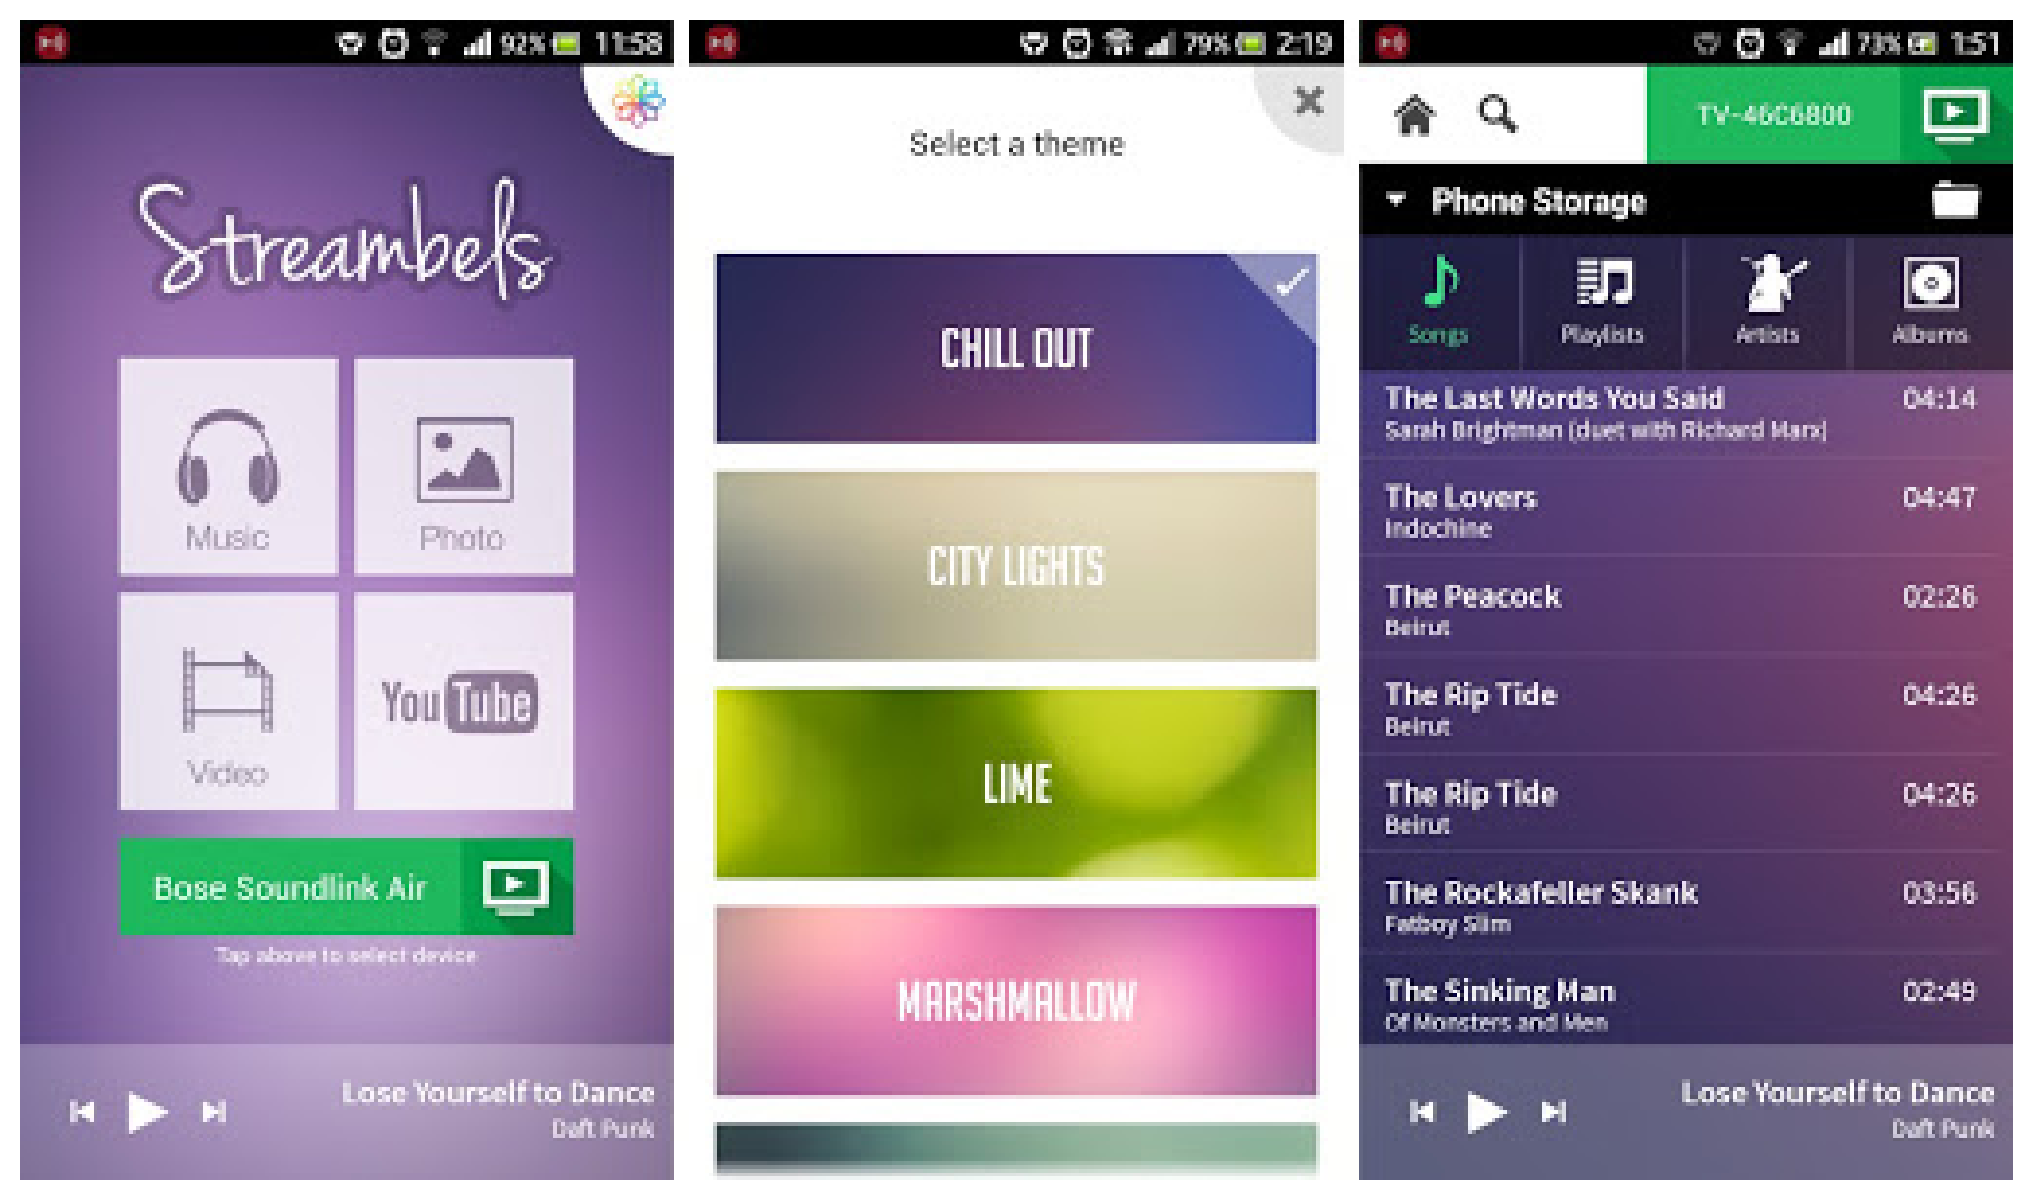
\includegraphics[height=9cm]{charts/streambels_ui}
\caption{Application UX design \label{chart5}}
\end{figure}

\subsection{Features}
As described previously that Airplay, DLNA and other standards work
differently and have different features, but according to the previous study,
we could combine some common use cases of both protocols.

The Android application we developed can handle most multimedia devices in 
a typical home networking. It has various features that make it a useful and
universal solution for multimedia home networking.

Firstly, the app itself is a multimedia playing, all media stored locally on the
phone storage and all media located in the home DLNA media servers can be
browsed and played on the phone.

Secondly, the app is fully compatible with AirPlay, DLNA, Chromecast and FireTV
receiver devices. 

Thirdly and most importantly, the application make the DLNA media server works
together with all kind of receivers regardless of protocol used. The app served
as a bridge of different multimedia receivers and media sources.

Last, YouTube and other on-line channels like Vimeo and Facebook are supported
as media source, and can be streamed regardless of protocol to all supported
receivers that are connected to home network.


\begin{itemize}
\item[--]Firstly the app is a multimedia player, it can play music, photos and videos 
on SD card locally on Android phone
\item[--]It can stream local content to Apple TV, Airport express and Airplay-enabled 
speakers.
\item[--]It can stream local content to DLNA media renderers, which has a huge device 
base.
\item[--]It can stream local content to Chromecast devices.
\item[--]It can browse content from the DLNA media servers, a typical source is a 
Network Attached Storage (NAS). And play the media locally on the Android device.
\item[--]It can browse content from the DLNA media servers and stream it to DLNA media 
renderers.
\item[--]It can browse content from DLNA media servers and stream it to Airplay enabled 
devices using a different protocol.
\item[--]It can proxy online channels' content to DLNA and Airplay enabled devices. 
(Currently YouTube and Facebook videos are supported, but integration to Spotify is still 
in progress).
\end{itemize}

\subsection{Extensibility}
In normal use cases, the data flow can be shown as figure \ref{chart4},
Streambels has embedded a media streaming server for local files and streaming
proxy for bridging the gap between online resources and home networking. By
using built-in proxy, Streambels is able to share on-line resources from
Internet to devices in home networking environment. New services and new
content providers can be easily added by just call the proxy interface.

The proxy system enables a huge extensibility possibility, which connects the
home networking and Internet or Cloud Services.

Further development abstracted all the protocols and developed an API for all
content holders or cloud services to integrate their service.

\subsection{Evaluation methodology}
Since the project is targeted to Android market, and is directly used by
end-users, feedback is really important to us for the continuous development. We
used Email for normal communication, user can edit feedback content directly
inside the application, and later content is sent to us by email.

There is no perfect application, so crash sometimes happen, thanks to Google,
the Google will help to collect the crash reports and show it inside developer
console.

Inside Streambels, we also used Google's Analytics API, which give us
great convenience to collect number of users and sessions every day. Other
information like operation system version, application version, active users
helped us to have insights into who are our users and how can we market for more
people in the world.

It is also interesting to see what kind of technologies are most used in their
daily life, thanks to Google's analytics SDK, we can trigger events when user
selected their receivers, so after months of statistics, we can figure out the
most popular standards and most popular online channels that user uses, and in
turn make better optimizations for users need.




\clearpage

\section{Results\label{chapter4}}

%% Results chapter
%% author Liu Peng

After designing, implementing and testing the application. We started several evaluation tests on the streaming performance. Finally we had released the application in Google Play Store in Nov 2013. So far, we have improved the application in many aspects and also brought many new features to it. During the past one year, we have accumulated many useful data and interesting results. In this chapter we will present and analyze those results.

\subsection{Performance}
In terms of streaming, our solution include two major streaming components. It would be helpful to study and compare which streaming protocol have the better performance while streaming multimedia contents. Moreover, by comparing different streaming types of media, we could investigate which protocol is best suitable for certain type of media. \\
\\Two major streaming technology we used in our solution are HTTP streaming and RTSP streaming.\\
\\
Hypertext Transfer Protocol (HTTP) refers to the protocol used to deliver web pages and images across the Internet worldwide. HTTP is an adopted, open standard and the most ubiquitous mode of delivery on-line. HTTP can be delivered by a variety of web servers, both commercial and open source.\\
\\
Real Time Streaming Protocol (RTSP) is a network control protocol used in entertainment and communications systems to control streaming media servers. RTSP is used to establish and control media sessions between two points, usually server and player client. Clients of media servers issue VCR-like commands, such as PLAY and PAUSE, to facilitate real-time control of playback of media files from the server. AirPlay uses RAOP, a RTSP-like streaming protocol, for the streaming of iTunes music. \\
\\
Since we have both protocols implemented in our application. We could compare the performance by streaming the same content to two receivers using different protocol. We selected a mp3 music file and try to stream it to an AirPlay Speaker and an DLNA Speaker, and we used Wireshark running on rooted Android phone to capture the packets in the network.\\
\\
The result is presented below, the initial packet count is relatively high. This is because there is a lot multicast messages in the network for device discovery. After that, streaming graph shows that after an initial increase in the traffic, network traffic enters a relatively stable state. This is because the TCP protocol reaches the best optimized transmission speed.\\
\\
Next, we added packet loss in the network and compare the influence to the two
streaming process. The result is shown in Figure \ref{airplay_vs_dlna_traffic}:\\
\begin{figure}
\hfill
\subfigure[AirPlay]{\includegraphics[width=7.2cm]{charts/oneMoreTime_airplay_android}}
\hfill
\subfigure[DLNA]{\includegraphics[width=7.2cm]{charts/oneMoreTime_dlna_android}}
\hfill
\caption{AirPlay vs DLNA streaming traffic
comparison \label{airplay_vs_dlna_traffic}}
\end{figure}

According to Figure \ref{airplay_vs_dlna_traffic}, the stream traffic for
AirPlay and DLNA streaming is very different. For AirPlay streaming, the traffic
growth is nearly linear, because the ROAP is a push like process, content can be
streamed in real time. However, for DLNA streaming, HTTP streaming is a pull
like process, the server fetches content from media server, so the content can
be buffered at the top network speed at the beginning of the playback.
Therefore, there is a short download period at the beginning of DLNA's
graph. \\ 
\\
Next, we try to limit the bandwidth and evaluate the performance change using
two solutions. We limited the bandwidth to 500kbps, 700kbps and 1000kbps
respectively and got Figure \ref{dlna_traffic_bw}:\\

\begin{figure}
\hfill
\subfigure[No
limit]{\includegraphics[width=7.2cm]{charts/oneMoreTime_dlna_android}}
\hfill
\subfigure[500kbps]{\includegraphics[width=7.2cm]{charts/oneMoreTime_dlna_android_bw_500k}}
\hfill
\subfigure[700kbps]{\includegraphics[width=7.2cm]{charts/oneMoreTime_dlna_android_bw_700k}}
\hfill
\subfigure[1000kbps]{\includegraphics[width=7.2cm]{charts/oneMoreTime_dlna_android_bw_1000k}}
\hfill
\caption{DLNA streaming traffic comparison in
bandwidth constrained situation\label{dlna_traffic_bw}}
\end{figure}



\begin{figure}
\hfill
\subfigure[No
limit]{\includegraphics[width=7.2cm]{charts/AirPlay_traffic_data}}
\hfill
\subfigure[5
percent loss]{\includegraphics[width=7.2cm]{charts/AirPlay_traffic_5loss_data}}
\hfill
\subfigure[10
percent loss]{\includegraphics[width=7.2cm]{charts/AirPlay_traffic_10loss_data}}
\hfill
\subfigure[15
percent loss]{\includegraphics[width=7.2cm]{charts/AirPlay_traffic_15loss_data}}
\hfill
\caption{AirPlay streaming performance in terms of packet loss \label{multiavp}}
\end{figure}


\begin{figure}
\hfill
\subfigure[No
limit]{\includegraphics[width=7.2cm]{charts/dlna_traffic_data}}
\hfill
\subfigure[5
percent loss]{\includegraphics[width=7.2cm]{charts/dlna_traffic_5loss_data}}
\hfill
\subfigure[10
percent loss]{\includegraphics[width=7.2cm]{charts/dlna_traffic_10loss_data}}
\hfill
\subfigure[15
percent loss]{\includegraphics[width=7.2cm]{charts/dlna_traffic_15loss_data}}
\hfill
\caption{DLNA streaming performance in terms of packet loss \label{multiavp}}
\end{figure}



\begin{figure}
\hfill
\subfigure[AirPlay
normal]{\includegraphics[width=7.2cm]{charts/AirPlay_traffic_data}}
\hfill
\subfigure[DLNA normal]{\includegraphics[width=7.2cm]{charts/dlna_traffic_data}}
\hfill
\subfigure[AirPlay
bad
network]{\includegraphics[width=7.2cm]{charts/badnetwork_AirPlay_traffic_data}}
\hfill
\subfigure[DLNA
bad network]{\includegraphics[width=7.2cm]{charts/badnetwork_dlna_traffic_data}}
\hfill
\caption{Comparison of AirPlay and DLNA in bad network conditions
\label{multiavp}}
\end{figure}


\subsection{Statistics}
Through 16 months' releasing, our application have achieved 924000 downloads from 223 countries all around the world, with around 10000 daily active users. This means our users almost cover 99% of the earth, a world map of our users is shown in Figure \ref{user_map}. So far, we got ratings from 10253 users, currently the average rating is 3.9 out of 5. The distribution is shown in Figure \ref{ratings}.

\begin{figure}[htb]
\centering \includegraphics[height=9cm]{charts/rating_distribution}
\caption{Rating distribution\label{ratings}}
\end{figure}

According to the rating distribution graph, most users are satisfied with our solution and gave 5 stars rating. However, the average rating is heavily influenced by the 1 star rating users. The reason of those unsatisfied users is that it happens that the receiver user have in home is not compatible with our application due to different reasons. It might be protocols are not supported yet, such as Roku box. Network condition problem also contributes to the incompatibility problem, some routers have by default disabled multicast due to security reasons. Another major cause of the incompatibility problem is that even use the same protocol, take DLNA for example, a minor implementation difference may cause the break of connection, thus, in the later phase, we have made receiver specific hacks to make our application work with most DLNA receivers regardless of which implementation they use.
In terms of user distribution, in 16 months, our application turns out to be popular in countries like France, United States, Germany, United Kingdom and Brazil. The user distribution is shown in Figure \ref{user_country}.
\begin{figure}[htb]
\centering \includegraphics[height=9cm]{charts/os_version_popularity}
\caption{Popularity of different Android versions \label{os_versions}}
\end{figure}

\begin{figure}[htb]
\centering \includegraphics[width=9cm]{charts/session_world_map}
\caption{World map of visits \label{user_map}}
\end{figure}

\begin{figure}[htb]
\centering \includegraphics[height=9cm]{charts/receiver_popularity}
\caption{Popularity of receiver types \label{receiver_types}}
\end{figure}

\begin{figure}[htb]
\centering \includegraphics[height=9cm]{charts/country_popularity}
\caption{Popularity in different countries \label{user_country}}
\end{figure}


\begin{figure}[htb]
\centering \includegraphics[height=9cm]{charts/sessions_per_day}
\caption{Sessions per day \label{sessions_perday}}
\end{figure}

\subsection{User study}
\begin{itemize}
\item[--]What information we can get back from users
\item[--]User behavior/ statistics
\item[--]Improve the application accordingly
\item[--]Strategies for decision making
\end{itemize}
Write result here.

\clearpage

\section{Conclusion\label{chapter5}}

%% Discussion chapter
%% author Liu Peng

The launch of Streambels has been successful, but the problem of multimedia home networking is still not completely solved. More manufacturers still keep developing and pushing new standards to the market. It is not possible to develop and support all the content sources and all the protocols in the future. To improve our solution and solve the problems of home networking, a better understanding and outlook of the future of home networking and accept new challenges.

\subsection{Further development}
\subsubsection{Support for more platforms}
The development on Android has been completed and achieved good result. The next step of developing is to make the solution also work on other platforms. Apple iOS and Microsoft Windows are the other two most popular mobile operating systems used by people. It is essential to firstly move on to iOS first since it has a larger user base. The work on iOS version implementation has already started, the first version currently is already released in the market, we are keep improving it to the same quality as Android version.
\subsubsection{Developing an Software Development Kit}
One of the limitations of our solution is that we can only work with limited content sources. There are thousands of content providers out there and it will be impossible to integrate with all content sources by ourselves. An ideal solution would to develop a Software Development Kit (SDK), so the content providers can directly integrate our solution in their software clients, enabling the access to the devices in home networking. Since the release of our Streambels, we have been actively developing this SDK. In the near future our solution will be used by more and more Internet content provides.
\subsubsection{Integration of receiver functionality}
Another limitation of our current solution is the content sharing between phones and tablets, sharing content between Android and iOS mobile platforms. In the further development, the receiver functionality is also planed to be integrated to our solution. By developing our own protocol using existing architecture, the compatibility can be guaranteed across different mobile platforms.
\subsubsection{Support for multi-session}
In our current solution, only one receiver device can be selected at the same time. However, there is a use case that user may want to stream the same item to different receiver at the same time. There is also a use case that different media items are needed to streamed to different receivers, the multi-session support becomes a valid demand. Further improvements should also take this demand into consideration, and integrate the support for multi-session streaming.
\subsubsection{Optimization for codec}
One big problem that is not solved of multimedia home networking is that the codec is quite different from device to device. Having aggregated all content sources, the application should also convert the format of content to a format that is supported by the receiver. In further development, the better transcoding support should be built in our solution.
\subsection{Future of multimedia home networking}
\subsubsection{Device discovery}
Given all the previous study about different standards in the market, there are mainly two mechanism of service discovery introduced: Simple Service Discovery Protocol(SSDP) and multicast DNS.  
\subsubsection{Information exchange}
RESTful will replace XML.
\subsubsection{Streaming protocol}
HTTP streaming will become main stream solution while RTSP will be used for real-time streaming.
\subsubsection{Internet of things}
More devices will be connected, more information will become available on the Internet.

\clearpage

%% L�hdeluettelo
%%
%% \phantomsection varmistaa, ett� hyperref-paketti latoo hypertekstilinkit
%% oikein.
%%
%% The \phantomsection command is nessesary for hyperref to jump to the 
%% correct page, in other words it puts a hyper marker on the page.

\phantomsection
%\addcontentsline{toc}{section}{Viitteet}
\addcontentsline{toc}{section}{References}

\bibliographystyle{unsrt}
\bibliography{reference} 

%\begin{thebibliography}{99}
%%% Reference chapter
%% author Liu Peng

%% Alla pilkun j�lkeen on pakotettu oikea v�li \<v�lily�nti>-merkeill�.
\bibitem{Kauranen} Kauranen,\ I., Mustakallio,\ M. ja Palmgren,\ V.
  \textit{Tutkimusraportin kirjoittamisen opas 
    .}  Espoo, Teknillinen korkeakoulu, 2006.

\bibitem{Itkonen} Itkonen,\ M. \textit{Typografian .} 3.\
  painos.  Helsinki, RPS-yht, 2007.

\bibitem{Koblitz} Koblitz,\ N. \textit{A Course in Number Theory and
    Cryptography. Graduate Texts in Mathematics 114.}  2.\ painos. New
  York, Springer, 1994.

%% Kun on useampi nimikirjain, jokaisen nimikirjaimen v�liin
%% kuuluu v�lily�nti. Oikea v�lin m��r� on saatu \<v�lily�nnill�>
\bibitem{bcs} Bardeen,\ J., Cooper,\ L.\ N. ja Schrieffer,\ J.\ R.
  Theory of Superconductivity. \textit{Physical Review,} 1957, vol.\
  108, nro~5, s.\ 1175--1204.

\bibitem{Deschamps} Deschamps,\ G.\ A. Electromagnetics and
  Differential Forms. \textit{Proceedings of the IEEE,} 1981, vol.\
  69, nro~6, s.\ 676--696.

%% Alla esimerkki englanninkielisen tavuttamisen pakottamisesta.
%% Oletusarvoisesti k�ytet��n suomalaista tavutusta, mutta viitteiss�
%% esiintyy usein muunkielisi� lauseita, jotka tulevat siten tavutetuksi
%% suomen kielen s��nt�jen mukaan. T�m�n voi korjata \foreignlanguage-
%% komennolla, jonka ensimm�inen parametri on vieraan kielen nimi ja toinen 
%% on vieraalla kielell� tavutettava teksti. 
\bibitem{Sihvola} Sihvola,\ A.\ et al.
  

%% Alla on suomalainen yhdistelm�sukunimi. Sen nimien v�liss� 
%% k�ytet��n yhdysmerkki� l. tavuviivaa, kirjoitetaan -.
\bibitem{Lindblom} Lindblom-,\ S. ja Wager,\ M.  Tieteellisten
   ohjaaminen. Teoksessa: Lindblom-Yl�nne,\ S. ja
  Nevgi,\ A. (toim.) \textit{Yliopisto- ja korkeakouluopettajan
    .}  Helsinki, WSOY, 2004, s.\ 314--325.
 
\bibitem{Miinusmaa} Miinusmaa,\ H. Neliskulmaisen rei�n poraamisesta
  kolmikulmaisella poralla. Diplomity�, Teknillinen korkeakoulu,
  konetekniikan osasto, Espoo, 1977.

%% T�ss� taas pakotettu englanninkielinen tavutus. 
%% Pedanttinen kirjoittaja pakottaa tietysti jokaiseen englanninkieliseen
%% lauseeseen englannin tavutuksen, mutta t�ss� esityksess� ei n�in ole
%% tehty selvyyden ja l�hdekoodin luettavuuden takia. 
\bibitem{Loh} Loh,\ N.\ C. High-Resolution Micromachined
  Interferometric Accelerometer. Master's Thesis, Massachusetts
  Institute of Technology, Cambridge,

\bibitem{Lonnqvist} ,\ A.
  

\bibitem{sfs} SFS 5342. Kirjallisuusviitteiden laatiminen. 2.\ painos.
  Helsinki, Suomen standardisoimisliitto, 2004. 20~s.

\bibitem{haastattelu} Palmgren,\ V. Suunnittelija. Teknillinen
  korkeakoulu, kirjasto. Otaniementie 9, 02150 Espoo. Haastattelu
  15.1.2007.

\bibitem{Ribeiro} Ribeiro,\ C.\ B., Ollila,\ E. ja Koivunen,\ V.
  

\bibitem{Stieber} Stieber,\ T. GnuPG Hacks. \textit{Linux Journal,}
  verkkolehti, 2006, maaliskuu, nro~143. Viitattu 19.1.2007. Lehti
  ilmestyy  painettuna. Saatavissa:
  \url{http://www.linuxjournal.com/article/8732.}

\bibitem{kone} Pohjois-Koivisto,\ T. Voiko kone tulevaisuudessa arvata
  tahtosi?  \textit{Apropos,} verkkolehti, helmikuu, nro~1, 2005.
  Viitattu 19.1.2007.  Saatavissa:
  \url{http://www.apropos.fi/1-2005/prima.php.}

\bibitem{Adida} Adida,\ B.  Advances in Cryptographic Voting Systems.
  Verkkodokumentti. Ph.D.\ Thesis, Massachusetts Institute of
  Technology, Cambridge, 

\bibitem{viittaaminen} ,\ P. WWW- viittaaminen
  . Verkkodokumentti.  26.11.2001.
  Viitattu 19.1.2007. Saatavissa:
  \url{http://www.cs.uku.fi/~kilpelai/wwwlahteet.html.}
%\end{thebibliography}

%% Liitteet
%% Appendices
\clearpage

%\appendix


%\phantomsection
%%
%% Lis�� tekstin "Liitteet" sis�llysluetteloon
%%
%% Adds the word "Appendices" to the table of contents
%\addcontentsline{toc}{section}{Liiteet}
%\addcontentsline{toc}{section}{Appendices}


%% if appendix is needed, uncomment below
%\section{Appendicy \label{AppendicyA}}

%%% Liitteiden kaavat, taulukot ja kuvat numeroidaan omana kokonaisuutenaan
%%
%% Equations, tables and figures have their own numbering in Appendices
\renewcommand{\theequation}{A\arabic{equation}}
\setcounter{equation}{0}  
\renewcommand{\thefigure}{A\arabic{figure}}
\setcounter{figure}{0}
\renewcommand{\thetable}{A\arabic{table}}
\setcounter{table}{0}


%% Verbatim-ymp�rist� ei muotoile tai tavuta teksti�. Fontti on monospace.
%% Verbatim-ymp�rist�n sis�ll� annettuja komentoja ei LaTeX k�sittele. 
%% Vasta \end{verbatim}-komennon j�lkeen jatketaan k�sittely�.
\begin{verbatim}
	this is not interpreted
	\clearpage
	\appendix
	\addcontentsline{toc}{section}{Liite A}
	\section*{Liite A}
	...
	\thispagestyle{empty}
	...
	ss
	...
	\clearpage
\end{verbatim}

Kaavojen numerointi muodostaa  oman kokonaisuutensa:
\begin{eqnarray}
d \wedge A  &=& F, \label{liitekaava1}\\
d \wedge F  &=& 0. \label{liitekaava2}
\end{eqnarray}

%\clearpage
%\section{Appendicy \label{AppendicyB}}

%%% Liitteiden kaavat, taulukot ja kuvat numeroidaan omana kokonaisuutenaan
%%
%% Equations, tables and figures have their own numbering in Appendices
\renewcommand{\theequation}{B\arabic{equation}}
\setcounter{equation}{0}  
\renewcommand{\thefigure}{B\arabic{figure}}
\setcounter{figure}{0}
\renewcommand{\thetable}{B\arabic{table}}
\setcounter{table}{0}

%%
%% Example of a figure, note the use of htb parameters which force
%% the figure to be inserted here
\begin{figure}[htb]
\begin{center}
\includegraphics[height=8cm]{charts/kuva2}
\end{center}
\caption{Kuvateksti, jossa on liitteen numerointi \label{liitekuva}}
\end{figure}
%%
Liitteiden taulukoiden numerointi on kuvien ja kaavojen kaltainen:
\begin{table}[htb]
\caption{Taulukon kuvateksti. \label{liitetaulukko}}
\begin{center}
\fbox{
\begin{tabular}{lp{0.5\linewidth}}
ds
\end{tabular}}
\end{center}
\end{table}
Kaavojen numerointi muodostaa  oman kokonaisuutensa:
\begin{eqnarray}
T_{ik} &=& -p g_{ik} + w u_i u_k + \tau_{ik},  \label{liitekaava3} \\
n_i    &=& n u_i + v_i.                        \label{liitekaava4}
\end{eqnarray}


\end{document}
